\documentclass{article}

\usepackage[margin=2cm]{geometry}
\usepackage{vwcol}
\usepackage[utf8x]{inputenc}
\usepackage[english,russian]{babel}
\usepackage{graphicx}

\sloppy
\begin{document}

\vwcolsetup{widths={0.3,0.7},sep=.5cm,justify=flush,rule=0pt,indent=1em, maxrecursion=100}
\begin{vwcol}
    \textbf{Ф617.} 
    \textit{Газетный текст фотографируется аппаратом «Зенит» c объективом, имеющим фокусное расстояние 50мм. дважды: \\1) c наименьшего допустимого для этого объектива a=0,5 м;\\2) после присоединения объектива к камере через удлинительное кольцо высотой h = 25 мм (таeже с минимально возможного расстояния). Найдите отношение размеров изображений, полученных на фотомплёнке в этих двух случаях.}
    \vspace{5cm}
    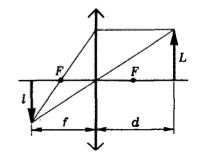
\includegraphics[width=0.29\textwidth]{image}
    \newpage
    So far while specifying the image file name in the  command we have omitted file extensions. However, that is not necessary, though it is often useful. If the file extension is omitted, LaTeX will search for any supported image format in that directory, and will search for various extensions in the default order (which can be modified).
    This is useful in switching between development and production environments. In a development environment (when the article/report/book is still in progress), it is desirable to use low-resolution versions of images (typically in .png format) for fast compilation of the preview. In the production environment (when the final version of the article/report/book is produced), it is desirable to include the high-resolution version of the images. 

\end{vwcol} 

\end{document}